\documentclass{article}

\PassOptionsToPackage{numbers,sort,compress}{natbib}
\makeatletter
\def\input@path{{../../}}
\makeatother
\usepackage[preprint]{neurips_2026}

\usepackage[utf8]{inputenc}
\usepackage[T1]{fontenc}
\usepackage{microtype}
\usepackage{graphicx}
\usepackage{booktabs}
\usepackage{tabularx}
\usepackage{multirow}
\usepackage{amsmath}
\usepackage{amssymb}
\usepackage{xcolor}
\usepackage{enumitem}
\usepackage{tikz}
\usepackage{url}
\usepackage{xspace}
\usepackage{hyperref}
\usetikzlibrary{arrows.meta,positioning,fit,calc}

\definecolor{automilblue}{HTML}{2D5F9A}
\definecolor{automilteal}{HTML}{2C7A7B}
\definecolor{automilgold}{HTML}{B7791F}
\definecolor{automilred}{HTML}{9B2C2C}
\definecolor{automilgray}{HTML}{4A5568}
\newcommand{\ours}{\textsf{autoMIL}\xspace}
\newcommand{\autobench}{\textsf{autobench}\xspace}
\newcommand{\unestablished}{\textcolor{automilred}{\textbf{not yet established}}}
\newcommand{\pendinginline}[2]{\textcolor{automilred}{\textbf{[PLACEHOLDER #1: #2]}}}
\newcommand{\pendingblock}[2]{%
  \begin{center}
  \fcolorbox{automilred}{automilred!4}{%
    \parbox{0.92\linewidth}{\textcolor{automilred}{\textbf{PLACEHOLDER #1.}} #2}}
  \end{center}}
\newcommand{\yes}{\textcolor{automilteal}{\textbf{yes}}}
\newcommand{\partialmark}{\textcolor{automilgold}{\textbf{partial}}}
\newcommand{\no}{\textcolor{automilgray}{\textbf{no}}}
\newcommand{\Rnative}{\mathcal{R}_{\mathrm{native}}}
\newcommand{\Rsearch}{\mathcal{R}_{\mathrm{search}}}

\title{\ours: Auditable Source-Level Research for Controlled Model Comparison}
\hypersetup{
  pdftitle={autoMIL: Auditable Source-Level Research for Controlled Model Comparison},
  pdfauthor={Shuolin Yin, Yeonwoo Seo, Jun Ma}
}

\author{%
  Shuolin Yin\thanks{Correspondence: \texttt{leo.yin@mail.utoronto.ca}. %
  \pendinginline{P-AUTH-1}{confirm final author list, order, and affiliations
  before public release.}}\\
  \And
  Yeonwoo Seo\\
  \And
  Jun Ma
}

\begin{document}

\maketitle

\begin{abstract}
A model leaderboard measures not only a method but also the training recipes,
debugging, and search effort invested in that method.
Coding agents can scale source-level research, yet their ability to edit and
execute repositories does not by itself make research effort attributable or
comparable across model families.
We introduce \ours, a research-operations system that stores parent-addressed
source overlays, reconstructs them in isolated git worktrees, accounts for
failure-inclusive launched attempts, and separates validation-guided selection
from held-out certification.
We use this system to define \autobench, a controlled audit of whether
pathology multiple-instance-learning rankings are stable when each published
method receives the same declared opportunity for autonomous source-level
research inside a method-identity contract.  The admissible search includes
executable train-only recipe programs while freezing each method's defining
mechanisms; cross-method ranking is the primary estimand and within-method lift
is explanatory.
The current implementation passes 51 selected contract tests, and an audited
static study record covers the declared 165-cell roster, but corrected
multi-seed search and sealed cross-arm certification are still outstanding;
this preprint therefore reports the framework, protocol, and present evidence
boundary rather than a premature ranking result.
\end{abstract}

\section{Introduction}

Leaderboards compress a research process into a number.  That number depends
on the model, but also on optimizer choice, learning-rate schedules, stopping
rules, data order, debugging, and the amount of search allocated to the model.
The importance of these choices is established: algorithm tunability differs
substantially across methods \cite{probst2019tunability}, and optimizer rankings
can change when hyperparameter-optimization opportunity is included in the
comparison \cite{schmidt2020optimizer}.  A nominally architecture-centered
benchmark can therefore measure a mixture of model quality and unequal research
effort.

Language-model agents make this confound larger.  MLAgentBench established
iterative file editing, code execution, and result inspection as an evaluation
setting \cite{huang2024mlagentbench}; AIDE formulates ML engineering as search
over candidate programs \cite{jiang2025aide}; and recent autonomous-research
systems perform tree-structured exploration under explicit execution budgets
\cite{yamada2025aiscientistv2,toledo2025aira,hambardzumyan2026aira2}.
Agent benchmarks increasingly save trajectories and use hidden evaluation
\cite{wijk2024rebench,zhang2025mlrcbench}.  These systems show that autonomous
source-level iteration is possible.  They do not, however, automatically
define the intervention needed to compare several existing published methods:
what constitutes a method-identity-preserving edit, what consumes the research budget,
which failures count, which result may guide the agent, and how the selected
descendant is certified.

\ours addresses this operations and evidence problem.  A proposed experiment
is not a mutable checkout or a prose claim; it is a node with an exact parent,
a source overlay, a declared intervention surface, execution metadata, and a
validation-visible result.  The system reconstructs that node at a pinned
commit, meters launched attempts even when they fail, and places held-out
metrics on a separate certification path.  Figure~\ref{fig:lifecycle} shows the
contract.  The proposal policy is replaceable: \ours is the substrate that
turns source-level interventions into attributable experimental evidence.

\begin{figure}[t]
\centering
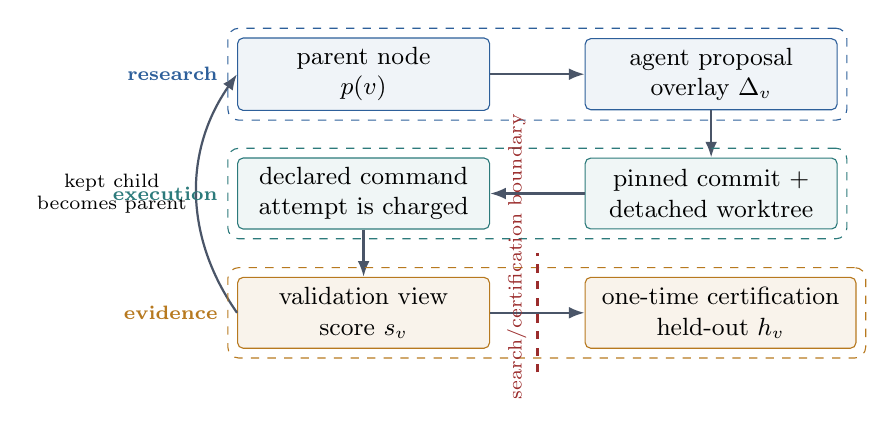
\begin{tikzpicture}[
  font=\small,
  node distance=6mm and 12mm,
  box/.style={draw, rounded corners=2pt, minimum height=9mm,
              minimum width=32mm, align=center, inner xsep=6pt, fill=white},
  research/.style={box, draw=automilblue, fill=automilblue!7},
  execution/.style={box, draw=automilteal, fill=automilteal!7},
  evidence/.style={box, draw=automilgold, fill=automilgold!9},
  arrow/.style={-{Latex[length=2mm]}, thick, draw=automilgray}
]
\node[research] (parent) {parent node\\$p(v)$};
\node[research, right=of parent] (proposal) {agent proposal\\overlay $\Delta_v$};
\node[execution, below=of proposal] (reconstruct) {pinned commit +\\detached worktree};
\node[execution, left=of reconstruct] (run) {declared command\\attempt is charged};
\node[evidence, below=of run] (val) {validation view\\score $s_v$};
\node[evidence, right=of val] (cert) {one-time certification\\held-out $h_v$};

\draw[arrow] (parent) -- (proposal);
\draw[arrow] (proposal) -- (reconstruct);
\draw[arrow] (reconstruct) -- (run);
\draw[arrow] (run) -- (val);
\draw[arrow] (val) -- (cert);
\draw[arrow, bend left=35] (val.west) to node[left,font=\scriptsize,align=center]{kept child\\becomes parent} (parent.west);

\node[fit=(parent)(proposal), draw=automilblue, dashed, rounded corners,
      label={[font=\scriptsize\bfseries,automilblue]left:research}] {};
\node[fit=(reconstruct)(run), draw=automilteal, dashed, rounded corners,
      label={[font=\scriptsize\bfseries,automilteal]left:execution}] {};
\node[fit=(val)(cert), draw=automilgold, dashed, rounded corners,
      label={[font=\scriptsize\bfseries,automilgold]left:evidence}] {};
\draw[automilred, very thick, dashed]
  ($(val.south east)!0.5!(cert.south west)+(0,-3mm)$) --
  ($(val.north east)!0.5!(cert.north west)+(0,3mm)$)
  node[above, pos=0.97, rotate=90, font=\scriptsize, text=automilred]
  {search/certification boundary};
\end{tikzpicture}
\caption{\textbf{The \ours lifecycle.}  Each intervention is attributable to a
parent and reconstructed from a source overlay.  Search receives the
validation-visible view; held-out fields are written to a separate
certification location and excluded from descendant overlays.  This is
framework-mediated non-interference for normal orchestrated execution, not an
operating-system security boundary against an adversarial same-user process.}
\label{fig:lifecycle}
\end{figure}

We make two contributions:
\begin{enumerate}[leftmargin=*,itemsep=2pt,topsep=2pt]
  \item \textbf{An auditable research-operations framework.}  \ours combines
  parent-addressed multi-file overlays, worktree reconstruction, declared file
  permissions, failure-inclusive attempt accounting, validation-only search,
  and separate held-out certification into one executable contract for
  repository-level autonomous research.
  \item \textbf{A controlled pathology-MIL ranking audit.}  \autobench asks
  whether a native/no-search cross-model ranking agrees with the ranking after
  every method receives a matched declared search opportunity.  Cross-arm
  ranking is essential; paired within-arm lift and anytime behavior explain
  any observed rank change or stability.  The final certified outcome is not
  claimed in this version.
\end{enumerate}

\section{From Agentic Search to a Controlled Comparison}
\label{sec:estimand}

\subsection{Research-opportunity estimand}

Let $a\in\mathcal{A}$ denote a published method class and
$c\in\mathcal{C}$ a study cell, such as a cohort, endpoint, encoder, and
aggregator combination.  An experiment node $v$ records a parent $p(v)$, a
source overlay $\Delta_v$, an execution specification, and a validation score
$s_v$.  If selected for final evaluation, the node also has a separately
revealed held-out result $h_v$.  A per-cell cap $B_c$ counts \emph{launched
attempts}; crashes, partial runs, and budget-killed jobs consume opportunity.
Usable completed or partial results are counted separately.

For each method, the consumer predeclares an identity contract $I_a$ over its
defining inference operator, forward branches, and core training/loss
mechanisms.  The admissible set $\mathcal{V}^{\mathrm{id}}_{a,c}$ preserves
$I_a$ while allowing both declared scalar configuration and executable
train-only recipe logic, including sampling, adaptive schedules,
optimizer/gradient policy, additive regularization, and stopping.  Candidates
that replace, delete, bypass, or zero a defining mechanism are outside this set
and cannot be reported as results for method $a$.

For each cell, the native/no-search regime selects the predeclared native
starting implementation and recipe.  The matched-search regime selects an
identity-preserving descendant using validation information subject to the same
declared attempt cap:
\begin{align}
  v^{0}_{a,c} &\in \mathcal{V}^{\mathrm{native}}_{a,c},\\
  v^{\star}_{a,c}(B_c)
      &= \arg\max_{v\in\mathcal{V}^{\mathrm{id}}_{a,c}:~
                   N_{\mathrm{launch}}(v)\leq B_c} s_v .
\end{align}
Certification produces two cross-method rankings,
\begin{equation}
  \Rnative(c)=\operatorname{rank}_{a}\!\left(h_{v^{0}_{a,c}}\right),\qquad
  \Rsearch(c;B_c)=\operatorname{rank}_{a}\!\left(h_{v^{\star}_{a,c}(B_c)}\right).
\end{equation}
The primary analysis is their agreement, displacement, and uncertainty across
cohorts.  The paired lift
$\Delta_{a,c}=h_{v^{\star}_{a,c}}-h_{v^{0}_{a,c}}$ is secondary: it explains
which methods moved and how much, but cannot replace the cross-arm ranking
comparison.

\subsection{What matched opportunity means}

Matching launches defines a reproducible intervention, not universal fairness.
It prevents a system from receiving extra replacements simply because its
proposals crash, but it does not equalize GPU-hours, wall-clock time, model
capacity, search difficulty, or the information content of one edit.  We
therefore use the narrower phrase \emph{matched launched-attempt opportunity}
and require a separate ledger of usable results, failure causes, elapsed time,
accelerator use, and language-model cost.  A time cap can be declared alongside
the launch cap, but neither should be silently converted into ``matched
successful evaluations.''

The baseline also answers a specific question.  Native recipes preserve how a
method is normally entered into the comparison; a single shared optimizer
would instead approximate an architecture-only ablation and can advantage
methods whose published training procedure already resembles the shared
recipe.  Native recipes must therefore be sourced component by component, and
benchmark-added choices must be labelled rather than presented as upstream
defaults.

\subsection{Closest prior work and the residual gap}

Table~\ref{tab:prior} positions the contribution against the closest agentic
systems and MIL infrastructure.  Source-level editing, experiment trees,
budgets, isolated execution, memory, and hidden evaluation are all prior art
\cite{huang2024mlagentbench,jiang2025aide,toledo2025aira,
hambardzumyan2026aira2,zhang2025mlrcbench,liu2026amid}.  Likewise,
PathBench-MIL and nnMIL provide substantial pathology-MIL pipeline and
benchmark infrastructure \cite{brussee2025pathbenchmil,luo2025nnmil}.  We do
not claim those ingredients individually.  The residual contribution is their
organization as a method-aware measurement instrument whose target is the
sensitivity of a \emph{cross-method ranking} to a controlled source-level
research intervention.

\begin{table}[t]
\centering
\caption{\textbf{Closest-prior comparison.} ``Repository'' means multi-file
source changes are the research object; ``lineage artifact'' means a selected
candidate is explicitly reconstructed from its parent and delta; ``final
separation'' means development selection is distinguished from held-out
evaluation.  The rightmost column is the target estimand, not a feature count.}
\label{tab:prior}
\scriptsize
\setlength{\tabcolsep}{3.2pt}
\begin{tabularx}{\linewidth}{lccccX}
\toprule
System & Repository & Lineage artifact & Explicit budget & Final separation &
Primary estimand \\
\midrule
MLAgentBench \cite{huang2024mlagentbench} & \yes & \no & \partialmark & \partialmark &
Agent performance on ML experimentation \\
AIDE \cite{jiang2025aide} & \partialmark & \yes & \partialmark & \partialmark &
Best candidate program \\
AIRA/AIRA2 \cite{toledo2025aira,hambardzumyan2026aira2} & \yes & \yes & \yes & \yes &
Research-agent search performance \\
MLRC-Bench \cite{zhang2025mlrcbench} & \yes & \partialmark & \yes & \yes &
Agent success on research challenges \\
AMID \cite{liu2026amid} & \yes & \partialmark & \yes & \yes &
Autonomous medical-model development \\
PathBench-MIL / nnMIL \cite{brussee2025pathbenchmil,luo2025nnmil} &
\partialmark & \no & \partialmark & \partialmark &
Configured pathology-MIL pipelines \\
\textbf{\ours + \autobench} & \yes & \yes & \yes & \yes &
\textbf{Cross-method rank response to matched source-level research} \\
\bottomrule
\end{tabularx}
\end{table}

\section{\ours}
\label{sec:system}

\subsection{Research layer: state before policy}

The experiment record is a directed tree rather than a flat table of terminal
scores.  A node points to its parent and stores only changed files, description,
status, resource metadata, and validation-visible metrics.  A child is proposed
against an explicit parent, so a result can be attributed to an exact research
step and reconstructed independently of the agent's conversation history.
Persistent trajectories can inform later proposals, but the search policy is
not fixed by the framework: a coding agent, heuristic proposer, or human can
operate the same state machine.

Keep/discard decisions are made on a predeclared validation composite and
margin.  Held-out results are not an axis of tree expansion.  This separation
is important because repeated validation-guided selection can already overfit;
allowing test feedback into the same loop would make the final comparison
uninterpretable.

\subsection{Execution layer: reconstruct, charge, collect}

For a queued node, the runner creates a detached git worktree at the recorded
base commit.  It validates overlay targets, rejects absolute paths, traversal,
and symlinks, optionally verifies SHA-256 digests, then copies only the
declared delta.  The consumer supplies the training command and result contract;
the orchestrator supplies process isolation, GPU masking, logging, and result
collection.

An attempt is charged when it is launched, before its scientific outcome is
known.  This ordering is deliberate.  If charging depended on a usable metric,
a brittle method implementation could obtain more proposals than a reliable one.
Completed and partial results are nevertheless tracked separately, because
matching launch opportunity without reporting yield would hide an important
property of the research process.  Orphan recovery is performed by the active
daemon rather than read-only status commands, avoiding accidental mutation of
live state.

\subsection{Evidence layer: declared permissions and born-sealed results}

The consumer declares editable and protected file surfaces.  Submission
hard-refuses a change that matches a protected path.  This contract is
file-based and intentionally keeps the generic framework free of
pathology-specific architecture knowledge.  The consumer owns the scientific
contract: for C2 it must protect each method's defining inference, forward, and
core-loss mechanisms, expose a guarded train-only recipe seam, and classify
every candidate as configuration-only, programmatic-recipe, identity-breaking,
or invalid.  Only the first two classes may enter the cross-method leaderboard.
The current framework enforces file declarations, but the per-arm semantic
invariants and runnable recipe seam remain implementation requirements.

Training writes a complete result to the node's certification directory before
placing a stripped, validation-visible result in the worktree.  Descendant
reconstruction excludes the certification subtree.  At the end of the study,
an explicit \texttt{certify} operation reveals the selected nodes' held-out
metrics once and warns that they must not be used for reselection.  This design
mediates the normal framework path; it is not a sandbox against arbitrary code
running under the same operating-system account.

\subsection{Consumer boundary and portability}

\ours does not create a task-specific training program.  A consumer supplies
four items: a runnable command, a result conforming to the validation/held-out
schema, a cell identity and budget, and editable/protected path declarations.
The framework repository contains no pathology-specific decision rule; the
\autobench package is a separate consumer.  Current evidence for this boundary
is structural plus a synthetic-consumer round trip.  It supports
consumer-agnostic mechanisms, not the stronger claim that arbitrary projects
require zero adaptation or that every execution backend has identical
production semantics.

\section{\autobench: A Pathology-MIL Ranking Audit}
\label{sec:autobench}

\subsection{Cohorts, tasks, and model regimes}

Whole-slide histology is a useful stress test for research-effort sensitivity:
slides contain many image patches, supervision is typically available only at
the patient or slide level, cohorts are modest, and training conventions differ
across MIL methods.  \autobench uses five cohorts from TCGA and CPTAC
\cite{tcga2013pancancer,wang2021gbm,cao2021pdac}.  Each cohort contributes one
classification endpoint and overall-survival prediction.  Table~\ref{tab:data}
records the current audited planning counts; final sample sizes and attrition
must be regenerated from frozen manifests before certification.

\begin{table}[t]
\centering
\caption{\textbf{Planned/audited cohort roster.}  Counts are study-planning
records, not a newly released cohort. HNSC has 431 cases, of which 414 are
currently gradeable. OS denotes overall survival.}
\label{tab:data}
\small
\setlength{\tabcolsep}{4.5pt}
\begin{tabularx}{\linewidth}{llXrr}
\toprule
Cohort & Source & Classification endpoint & Cases & OS deaths \\
\midrule
LUAD & TCGA & KRAS mutation (binary) & 465 & 167 \\
LGG & TCGA & IDH1 mutation (binary) & 491 & 115 \\
GBM & CPTAC & TP53 mutation (binary) & 99 & 72 \\
PDAC & CPTAC & immune subtype (3-class) & 105 & 81 \\
HNSC & TCGA & tumour grade (3-class) & 431 (414) & 205 \\
\bottomrule
\end{tabularx}
\end{table}

The tile-level grid crosses three pathology foundation-model encoders---UNI
v2, Virchow2, and H-Optimus-1
\cite{xu2024uni,vorontsov2024virchow,saillard2024hoptimus}---with four
published aggregator methods: CLAM \cite{lu2021clam}, nnMIL SimpleMIL
\cite{luo2025nnmil}, attention MIL \cite{ilse2018attention}, and DTFD-MIL
\cite{zhang2022dtfd}.  TITAN \cite{ding2024titan} is reported as a separate
slide-level regime because it jointly defines the representation and
aggregation route; it is not another cell in the tile-encoder by aggregator
factorial design.

With five cohorts, the declared roster contains 65 classification experiments
and 100 survival experiments.  The survival count is larger because SimpleMIL,
ABMIL, and TITAN are evaluated with two predeclared survival objectives where
supported.  This 165-cell roster is a controlled sample of pathology MIL, not
an exhaustive field leaderboard: prominent alternatives such as DSMIL and
TransMIL are outside the current four-aggregator set
\cite{li2021dsmil,shao2021transmil}.

\pendingblock{P-GBM-1}{Confirm whether CPTAC-GBM survival remains in the
certified roster, is retained only as a labelled low-signal sensitivity case,
or is removed before the roster is frozen. The 165-cell count and all
denominators must be regenerated if this decision changes.}

\subsection{Native/no-search and matched-search regimes}

Figure~\ref{fig:audit} shows the comparison.  For the native/no-search arm,
each framework begins from its upstream architecture and sourceable native
recipe.  Every component is labelled as upstream-declared, conditionally
derived from an upstream rule, or benchmark-added.  For the matched-search arm,
a coding agent may propose source and recipe edits only within the declared
method-identity contract and under the same launched-attempt opportunity in
each comparison cell.  This is not a scalar-only menu: admissible
programmatic-recipe candidates may implement train-only sampling, adaptive
schedules, optimizer or gradient policy, additive regularization, and stopping.
They may not replace inference operators, introduce a new learnable forward
branch, or remove a defining core training mechanism.  Correctness fixes update
the common protocol and trigger affected baseline regeneration; they are not
counted as agent lift.

\pendingblock{P-BASE-1}{Confirm the headline baseline policy. The present prose
assumes per-method upstream/native recipes as the primary no-search ranking;
if a standardized shared-recipe ranking is primary or co-primary, revise
Sections~2.2 and 4.2 and preregister how unsupported framework--recipe
combinations are handled.}

\begin{figure}[t]
\centering
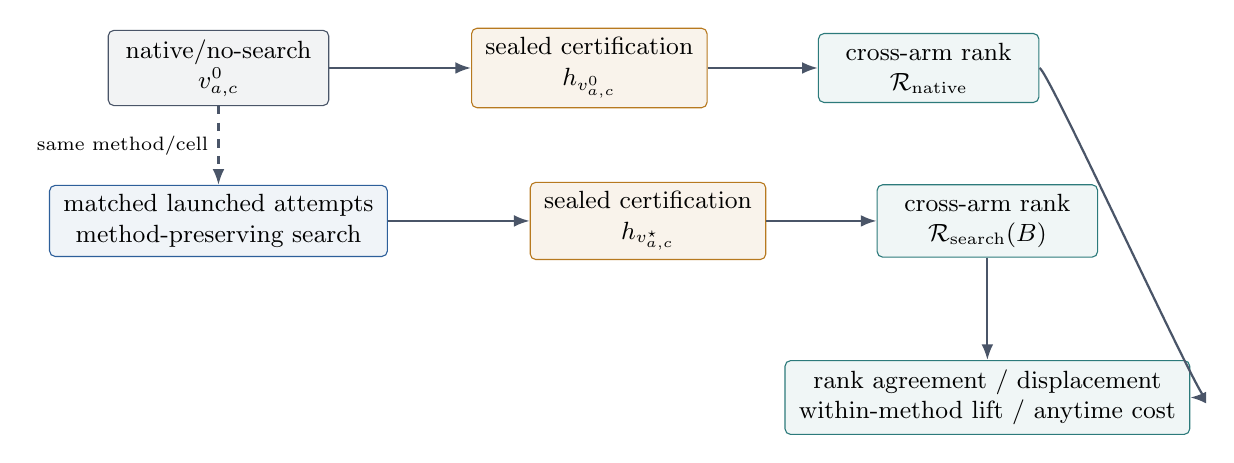
\begin{tikzpicture}[
  font=\small,
  node distance=6mm and 9mm,
  box/.style={draw, rounded corners=2pt, align=center, minimum height=8mm,
              minimum width=28mm, inner xsep=5pt},
  native/.style={box, draw=automilgray, fill=automilgray!7},
  search/.style={box, draw=automilblue, fill=automilblue!7},
  cert/.style={box, draw=automilgold, fill=automilgold!9},
  outputbox/.style={box, draw=automilteal, fill=automilteal!7},
  arrow/.style={-{Latex[length=2mm]}, thick, draw=automilgray}
]
\node[native] (native) {native/no-search\\$v^0_{a,c}$};
\node[search, below=10mm of native] (budget) {matched launched attempts\\method-preserving search};
\node[cert, right=18mm of native] (cert0) {sealed certification\\$h_{v^0_{a,c}}$};
\node[cert, right=18mm of budget] (cert1) {sealed certification\\$h_{v^\star_{a,c}}$};
\node[outputbox, right=14mm of cert0] (rank0) {cross-arm rank\\$\Rnative$};
\node[outputbox, right=14mm of cert1] (rank1) {cross-arm rank\\$\Rsearch(B)$};
\node[outputbox, below=13mm of rank1] (paired) {rank agreement / displacement\\within-method lift / anytime cost};

\draw[arrow] (native) -- (cert0);
\draw[arrow] (budget) -- (cert1);
\draw[arrow] (cert0) -- (rank0);
\draw[arrow] (cert1) -- (rank1);
\draw[arrow] (rank0.east) .. controls +(1mm,0) and +(1mm,0) .. (paired.east);
\draw[arrow] (rank1.south) -- (paired.north);
\draw[arrow, dashed] (native) -- node[left,font=\scriptsize]{same method/cell} (budget);
\end{tikzpicture}
\caption{\textbf{Controlled ranking audit.}  Native and searched descendants
are certified on the same held-out split.  The two cross-arm rankings are the
primary objects.  Paired lift, failure yield, and anytime cost explain the
ranking response but do not replace it.  The schematic is result-neutral.}
\label{fig:audit}
\end{figure}

This admissibility rule is settled before outcomes are observed, but its current
implementation is incomplete.  File-level permissions alone do not prevent a
flag or loss weight from deleting a defining mechanism, and the declared
structured policy path cannot yet execute the required train-only recipe
programs.  Identity-breaking candidates may be archived as evolved descendants,
but they are excluded from C2 and never attributed to the published method.

\pendingblock{P-METHOD-1}{Implement and test the settled method-identity
contract before launching search: symmetric protected core files,
machine-readable per-arm invariants, a consumer-side programmatic RecipePolicy
hook called by protected trainers, and persistent four-way candidate
classification.}

\subsection{Metrics, selection, and inference}

Classification is reported with one-vs-rest macro AUC as the primary metric and
balanced accuracy as a complementary class-sensitive metric.  Survival is
reported separately with concordance; classification and survival are never
pooled into one performance number.  Five-fold splits are patient-stratified,
and all competing arms within a cohort use the same patient partitions.
Validation composites control search and promotion; held-out predictions and
metrics enter only through certification.

The inferential unit cannot be the nominal set of 165 cells.  Cells from the
same cohort share patients and folds, and several cells also share
representations.  The final analysis will therefore report cohort-level
rankings and paired model comparisons, then aggregate only with a declared
dependence-aware procedure.  Patient-level paired bootstrap intervals can
quantify metric and rank uncertainty within a certified seed; repeated
initialization seeds are needed to characterize training variability.
Prior pathology-MIL evidence reports test-AUC swings of 10--15 points from
initialization, batch order, and learning rate, and cautions that validation
AUC may not predict test AUC reliably \cite{mammadov2025variability}.  Because
the current campaign record is single-seed, this version makes no statistical
significance or seed-robust ranking claim.

\pendingblock{P-SEED-1}{Confirm whether the preprint remains a descriptive
single-seed audit or adds a repeated-seed confirmatory set. Until confirmed,
retain no significance, stability, or seed-robustness claim.}

\subsection{Evidence and resource ledger}

A certifiable comparison must release more than a leaderboard.  For each
method and cell, the evidence ledger includes: upstream commit and native
recipe sources; benchmark-added components; frozen splits and feature
identifiers; every parent-linked overlay; validation trajectories; selected
nodes; launched and usable attempt counts; failures; wall-clock, GPU, and
language-model costs; candidate admissibility class; and the one-time held-out
result.  This ledger makes an informative null possible.  If rankings remain
stable, the record shows the research intervention under which stability was
observed; if they move, it locates the edits, costs, and methods responsible.

\section{Validation and Current Evidence}
\label{sec:validation}

We separate locally verified framework behavior from cluster-audit records and
from outcomes that do not yet exist.  This distinction is central to the
preprint: protocol maturity is evidence, but it is not a substitute for the
certified C2 result.

\subsection{Does the framework enforce its contract?}

A focused regression run executed 51 tests covering the worktree runner,
born-sealed result path, launched-attempt cap, evaluation accounting, protected
files, framework purity, and a synthetic-consumer round trip.  All 51 passed in
4.80 seconds on the current checkout (Table~\ref{tab:validation}).  These tests
directly exercise the named C1 mechanisms.  They do not prove operating-system
security, production equivalence among execution backends, or scientific
generality.

\begin{table}[t]
\centering
\caption{\textbf{Current framework validation.}  This is a selected invariant
suite, not a claim that the full workspace dependency matrix is green.}
\label{tab:validation}
\small
\begin{tabularx}{\linewidth}{XrX}
\toprule
Invariant family & Result & Scope of evidence \\
\midrule
Worktree reconstruction and safe overlay application & pass &
Pinned checkout, digest/path handling, collection \\
Born-sealed validation/certification path & pass &
Split result write and descendant exclusion \\
Launch-cap and usable-result accounting & pass &
Failure-inclusive attempts, separate usable counts \\
Consumer-declared protected files & pass &
Submission refusal for declared paths \\
Framework purity and synthetic consumer & pass &
No pathology mechanism in core; one toy consumer \\
\midrule
\textbf{Selected total} & \textbf{51/51} & \textbf{4.80 s, current checkout} \\
\bottomrule
\end{tabularx}
\end{table}

\subsection{Is the static study substrate usable?}

The external cluster audit reports 195 stored experiments, comprising every
cell in the canonical 165-cell roster plus 30 off-roster LUAD experiments.
Across 8,440 per-fold records it reports no fold-count anomaly and no non-finite
value in the primary AUC, balanced-accuracy, or concordance fields.  The
underlying cluster artifacts are not present in this local checkout, so these
are audited execution records rather than locally reproduced results.

The same audit exposed a consequential provenance defect: 102 of 195 serialized
configuration files describe a generic recipe rather than the recipe that
actually executed.  Runtime provenance reconstruction is therefore the
required source for historical recipes, and corrected native baselines must be
regenerated before a leaderboard is published.  We deliberately omit a rerun
count because current planning documents disagree; the canonical roster and
runtime provenance must be joined mechanically.

A separate implementation blocker remains in the CLAM survival path: it
hard-codes AdamW while exposing the optimizer as a declared searchable field.
An agent can therefore request a different optimizer and have the request
silently ignored.  This defect must be repaired and regression-tested before
the matched campaign; none of the current text treats the affected runs as
search-fidelity evidence.

\subsection{Are the no-search baselines obvious strawmen?}

A validation-only triage screen was available for 174 gradeable roster
experiments.  Relative to task-specific chance thresholds, 151 were more than
0.05 above chance, 19 were within 0.05, and four were at or below chance.  All
four subchance runs and 13 of the 20 near-chance cases were concentrated in GBM
survival.  This finding is useful but narrow: it argues against a globally
broken study substrate and flags GBM survival as a predefined low-signal case.
It does not establish that recipes are optimal, that the native ranking is
unbiased, or that any model is superior.  No held-out value was used for this
screen.

\subsection{What remains unestablished}

Table~\ref{tab:status} states the current evidence boundary.  In particular,
this preprint does not report a rank flip, rank stability, or a winning model.
Those statements require corrected baselines, method-identity enforcement, a
runnable programmatic-recipe channel, the matched campaign, repeated seeds,
dependence-aware analysis, and one-time certification.

\begin{table}[t]
\centering
\caption{\textbf{Evidence status for C2 as of 30 July 2026.}  ``Reported''
denotes an external cluster-audit record whose raw artifacts are not in this
checkout.}
\label{tab:status}
\scriptsize
\setlength{\tabcolsep}{4pt}
\begin{tabularx}{\linewidth}{l l X X}
\toprule
Object & Status & Evidence now & Required to unlock the claim \\
\midrule
Canonical roster & reported & 165/165 cells within 195 stored runs &
Frozen manifest plus local artifact release \\
Fold/metric integrity & reported & 8,440 records; no primary non-finite value &
Re-run audit over released artifacts \\
Baseline viability & reported & validation-only 151/174 exceeded chance by $>0.05$ &
Correct native recipes and held-out certification \\
Native cross-arm ranking & \unestablished & historical configs misstate recipes &
Canonical provenance join and corrected reruns \\
Matched-search ranking & \unestablished & protocol and framework only &
Method invariants, recipe channel, matched search, seed ledger, certification \\
Rank stability/change & \unestablished & no certified paired rankings &
Dependence-aware comparison of both rankings \\
\bottomrule
\end{tabularx}
\end{table}

\subsection{Certified cross-arm results}

\pendingblock{P-RESULT-1}{Insert the frozen native/no-search and matched-search
cross-arm ranking table or figure only after canonical provenance
reconciliation, selected-node freezing, and one-time held-out certification.
Report classification and survival separately, with TITAN labelled as a
different regime.}

\pendingblock{P-RESULT-2}{Insert rank agreement/displacement and paired
within-method lift with patient/cohort-aware uncertainty. Within-method lift
must explain the cross-arm result; it must not replace the ranking comparison.}

\pendingblock{P-RESULT-3}{Insert anytime curves and the resource/failure ledger:
launched attempts, usable outcomes, crash and budget-kill counts, wall-clock,
GPU-hours, and language-model cost.}

\section{Discussion and Limitations}

\paragraph{The novelty is the measurable question, not the ingredients.}
Worktrees, experiment graphs, resource caps, validation selection, and hidden
tests all have clear precedents.  \ours contributes their executable
coordination around a different estimand: how an existing cross-method ranking
responds when autonomous source-level research opportunity is declared,
matched, and attributable.  C2 is therefore not an optional demo.  It is the
scientific test that gives the integrated C1 contract meaning.

\paragraph{Internal validity.}
Five issues can invalidate the audit.  First, historical configs do not
faithfully encode every executed baseline recipe.  Second, a permissive edit
surface can transform one model family into another, while a scalar-only menu
would fail to instantiate the intended source-level research opportunity.
Third, single-seed training cannot distinguish a search effect from
initialization variance.  Fourth, validation-guided search can overfit even when
test data remain sealed.  Fifth, shared patients and folds make cell-level
independence false.  The corresponding remedies are, respectively,
runtime-provenance reconstruction; per-method invariants plus a guarded
programmatic train-only recipe seam; repeated seeds; one-time certification;
and cohort/patient-aware paired analysis.

\paragraph{External validity.}
The benchmark covers five cohorts, three patch encoders, four tile-aggregator
methods, and one separate slide-level model.  It does not represent all
pathology tasks or model families.  The framework core contains no
pathology-specific mechanism and passes one synthetic-consumer test, but this
is not evidence for zero-effort adoption in arbitrary repositories.  Local,
SLURM, and Ray interfaces exist; real production-equivalence evidence across
those backends remains outstanding.

\paragraph{Security and governance.}
The result firewall assumes normal execution through the orchestrator.  Code
with same-user filesystem access is outside the threat model.  Moreover, an
agent can exploit a poorly declared consumer surface without violating a
framework rule.  Protected inputs, splits, metric code, and method-defining
components must therefore be reviewed as part of the study protocol.  The
framework records and enforces declarations; it cannot infer the scientific
meaning of every source edit.

\paragraph{Outcome-neutral value.}
A stable ranking would show robustness to the declared research intervention,
not that all recipe bias is absent.  A changed ranking would quantify
sensitivity under this budget, not establish a universally superior model.
Either outcome is informative if accompanied by the intervention and resource
ledger.  Neither is informative if baselines, method identity, failures, or
test exposure are repaired after inspecting the final result.

\subsection{Conclusion}

\ours is a framework for turning repository-level coding-agent interventions
into reconstructable, parent-linked experimental evidence.  Its current
implementation mediates declared source permissions, failure-inclusive launch
budgets, validation-only search signals, and a distinct held-out certification
path.  Focused invariant tests support those mechanisms, while their limits are
explicit: the system is an auditable operations contract, not an
operating-system sandbox or a proof of scientific generality.

\autobench uses that contract to ask whether pathology-MIL cross-model rankings
survive matched autonomous research opportunity.  That cross-arm comparison is
the second main contribution; within-arm lift explains it.  The static roster
and validation-only screen are sufficiently mature to expose baseline and
inference problems, but the final answer awaits corrected native recipes,
method-identity enforcement, the programmatic-recipe channel, repeated-seed
evidence, and sealed certification.  This
preprint fixes the question and the evidence standard before revealing the
outcome.

\section*{Broader Impact}

Auditable experiment lineages can make autonomous ML research easier to inspect,
reproduce, and challenge.  They may also accelerate the production of
seemingly authoritative comparisons.  In computational pathology, premature
leaderboards can redirect clinical-research effort even when the underlying
cohorts are small or unrepresentative.  We therefore keep patient-level data
outside the release, separate validation from certification, disclose failed
runs and compute, and avoid clinical-performance claims.  \ours is intended for
research operations; it does not validate a model for patient care.

\bibliographystyle{unsrtnat}
\bibliography{references}

\clearpage
\appendix

\section{Operational Contract}
\label{app:contract}

\paragraph{Result schema.}
A training process emits a status, validation-visible metric dictionary,
validation-derived composite, elapsed time, peak memory, and an optional
held-out block.  The orchestrated writer places the full object under the
certification directory and removes held-out fields from the worktree copy.
The orchestrator, not the training script, writes the global result table.

\paragraph{Attempt semantics.}
The comparison cap increments on launch.  Completed, partial, crashed,
budget-killed, and cancelled outcomes remain distinguishable.  A partial
result can be scientifically usable but never refunds the launch that produced
it.  Per-cell reports must show at least launched attempts, usable outcomes,
failure categories, wall time, accelerator-hours, and language-model spend.

\paragraph{Submission and reconstruction.}
Overlay paths must be relative to the project, remain within the project root,
and not be symlinks.  Consumer-declared protected paths are rejected at
submission.  Reconstruction starts from a pinned commit and can verify stored
digests before applying the overlay.  Certification files are excluded from
descendant reconstruction.

\section{Reproduction Status and Commands}
\label{app:repro}

The focused validation reported in Table~\ref{tab:validation} was run from the
repository root with:
\begin{verbatim}
.venv/bin/pytest tests/test_runner.py \
  tests/test_born_sealed_firewall.py \
  tests/test_launch_cap_enforcement.py \
  tests/test_daemon_eval_accounting.py \
  tests/test_submit_protected_files.py \
  tests/test_framework_purity.py \
  tests/test_synthetic_consumer_roundtrip.py -q
\end{verbatim}
It produced \texttt{51 passed in 4.80s}.  We did not use the full workspace as a
green validation gate: collection in the present local environment reported
856 collected tests and 114 collection errors, principally outside the focused
contract command.  The paper consequently makes only the selected-test claim.

The local checkout does not contain the cluster result tree underlying the
195-run audit.  Releasing or mounting that tree and running a versioned audit
reader are prerequisites for independently reproducing the reported static
counts.  The final campaign should additionally publish the exact environment,
accelerator type, per-run timing, total compute, language-model/runtime
versions, prompts or skills, and every selected source overlay.

\pendingblock{P-ARTIFACT-1}{Add the permanent code/release URL, version or
commit, environment lockfile, cluster artifact location, data/feature access
instructions, asset licenses, and final compute/LLM-cost ledger.}

\section{Planned Confirmatory Analysis}
\label{app:analysis}

The following analysis must be frozen before final certification:
\begin{enumerate}[leftmargin=*]
  \item regenerate the canonical roster from dataset manifests and join every
  native result to runtime provenance;
  \item repair the CLAM survival optimizer path so every declared search field
  controls the executed recipe, then add a regression test for silent drops;
  \item implement and test per-method defining-mechanism invariants, symmetric
  protected cores, the consumer-side programmatic \texttt{RecipePolicy} seam,
  and four-way candidate classification;
  \item execute matched launch caps with failures and resources retained;
  \item repeat selected native and searched nodes across predeclared seeds;
  \item certify native and searched selections once on identical held-out
  patient splits;
  \item report cohort-specific cross-arm rankings, rank agreement and
  displacement, paired within-method lift, anytime curves, and patient/seed
  uncertainty without treating 165 cells as independent.
\end{enumerate}
TITAN remains a labelled slide-level regime and is not silently pooled with the
tile-encoder by aggregator factorial ranking.

\section{Author and Tooling Disclosure}

The authors designed the framework, benchmark, contribution hierarchy, and
evidence boundaries.  Language models are an object of study because coding
agents propose source-level experiments.  Language-model assistance was also
used to organize and edit this manuscript; all factual claims, citations,
source anchors, and reported test commands remain the authors'
responsibility.  No generated empirical value or mock result figure is used in
the paper.

\input{../../checklist}

\end{document}
